%\documentclass[a4paper]{article}

\usepackage[spanish, es-tabla, es-noshorthands]{babel}
\usepackage[table,xcdraw]{xcolor}
\usepackage[a4paper, footnotesep=1.25cm, headheight=1.25cm, top=2.54cm, left=2.54cm, bottom=2.54cm, right=2.54cm]{geometry}
%\geometry{showframe}

%\usepackage{wrapfig}			%Wrap figure in text
\usepackage[export]{adjustbox}	%Move images
\usepackage{changepage}			%Move tables

\usepackage{tikz}
\usepackage{amsmath}
\usepackage{amsfonts}
\usepackage{amssymb}
\usepackage{float}
\usepackage{graphicx}

\usepackage{caption}
\usepackage{subcaption}
\usepackage{multicol}
\usepackage{multirow}
\usepackage{wrapfig}
\setlength{\doublerulesep}{\arrayrulewidth}
\usepackage{booktabs}
\usepackage[numbib, nottoc, notlot, notlof]{tocbibind}

\usepackage{hyperref}
\hypersetup{
    colorlinks=true,
    linkcolor=blue,
    filecolor=magenta,      
    urlcolor=blue,
    citecolor=blue,    
}

%Change Font Size

% #1 = size, #2 = text
\newcommand{\setparagraphsize}[2]{{\fontsize{#1}{6}\selectfont#2 \par}}		%Cambia el size de todo el parrafo
\newcommand{\setlinesize}[2]{{\fontsize{#1}{6}\selectfont#2}}				%Cambia el font de una oración

\newcommand{\note}[1]{
	\begin{center}
		\huge{ \textcolor{red}{#1} }
	\end{center}
}

%FONTS (IMPORTANTE): Compilar en XeLaTex o LuaLaTeX
\usepackage{anyfontsize}	%Font size
\usepackage{fontspec}		%Font type

\usepackage{etoolbox}
\usepackage{todonotes}

\newcommand{\observacion}[2]{  \ifnumequal{1}{#1}{ { \todo[inline,backgroundcolor=red!25,bordercolor=red!100]{\textbf{Observación: #2}} } }{  }  }

\setcounter{topnumber}{2}
\setcounter{bottomnumber}{2}
\setcounter{totalnumber}{4}
\renewcommand{\topfraction}{0.85}
\renewcommand{\bottomfraction}{0.85}
\renewcommand{\textfraction}{0.15}
\renewcommand{\floatpagefraction}{0.8}
\renewcommand{\textfraction}{0.1}
\setlength{\floatsep}{5pt plus 2pt minus 2pt}
\setlength{\textfloatsep}{5pt plus 2pt minus 2pt}
\setlength{\intextsep}{5pt plus 2pt minus 2pt}

\newcommand{\quotes}[1]{``#1''}
\usepackage{array}
\newcolumntype{C}[1]{>{\centering\let\newline\\\arraybackslash\hspace{0pt}}m{#1}}
\usepackage[american]{circuitikz}
\usetikzlibrary{calc}
\usepackage{fancyhdr}
\usepackage{units} 



\pagestyle{fancy}
\fancyhf{}
\lhead{IA.03 - Inteligencia Artificial}
\rhead{Lambertucci, Mestanza}
\rfoot{Página \thepage}

\usepackage{listings}

\usepackage{color} %red, green, blue, yellow, cyan, magenta, black, white
\definecolor{mygreen}{RGB}{28,172,0} % color values Red, Green, Blue
\definecolor{mylilas}{RGB}{170,55,241}
%Items con bullets y no cuadrados
\renewcommand{\labelitemi}{\textbullet }
\lstset{language=R,%
    %basicstyle=\color{red},
    breaklines=true,%
    morekeywords={matlab2tikz},
    keywordstyle=\color{blue},%
    morekeywords=[2]{1}, keywordstyle=[2]{\color{black}},
    identifierstyle=\color{black},%
    stringstyle=\color{mylilas},
    commentstyle=\color{mygreen},%
    showstringspaces=false,%without this there will be a symbol in the places where there is a space
    numbers=left,%
    numberstyle={\tiny \color{black}},% size of the numbers
    numbersep=9pt, % this defines how far the numbers are from the text
    emph=[1]{for,end,break},emphstyle=[1]\color{red}, %some words to emphasise
    %emph=[2]{word1,word2}, emphstyle=[2]{style},    
    literate=
    	{á}{{\'a}}1 {é}{{\'e}}1 {í}{{\'i}}1 {ó}{{\'o}}1 {ú}{{\'u}}1
  		{Á}{{\'A}}1 {É}{{\'E}}1 {Í}{{\'I}}1 {Ó}{{\'O}}1 {Ú}{{\'U}}1
		{à}{{\`a}}1 {è}{{\`e}}1 {ì}{{\`i}}1 {ò}{{\`o}}1 {ù}{{\`u}}1
  		{À}{{\`A}}1 {È}{{\'E}}1 {Ì}{{\`I}}1 {Ò}{{\`O}}1 {Ù}{{\`U}}1
  		{ä}{{\"a}}1 {ë}{{\"e}}1 {ï}{{\"i}}1 {ö}{{\"o}}1 {ü}{{\"u}}1
  		{Ä}{{\"A}}1 {Ë}{{\"E}}1 {Ï}{{\"I}}1 {Ö}{{\"O}}1 {Ü}{{\"U}}1
  		{â}{{\^a}}1 {ê}{{\^e}}1 {î}{{\^i}}1 {ô}{{\^o}}1 {û}{{\^u}}1
  		{Â}{{\^A}}1 {Ê}{{\^E}}1 {Î}{{\^I}}1 {Ô}{{\^O}}1 {Û}{{\^U}}1
  		{Ã}{{\~A}}1 {ã}{{\~a}}1 {Õ}{{\~O}}1 {õ}{{\~o}}1
  		{œ}{{\oe}}1 {Œ}{{\OE}}1 {æ}{{\ae}}1 {Æ}{{\AE}}1 {ß}{{\ss}}1
  		{ű}{{\H{u}}}1 {Ű}{{\H{U}}}1 {ő}{{\H{o}}}1 {Ő}{{\H{O}}}1
  		{ç}{{\c c}}1 {Ç}{{\c C}}1 {ø}{{\o}}1 {å}{{\r a}}1 {Å}{{\r A}}1
  		{€}{{\euro}}1 {£}{{\pounds}}1 {«}{{\guillemotleft}}1
  		{»}{{\guillemotright}}1 {ñ}{{\~n}}1 {Ñ}{{\~N}}1 {¿}{{?`}}1,
  	inputencoding=latin1,
}

%\begin{document}
%
\subsection{Consigna}
\begin{itemize}
\item Primera Parte Ejercicio 1 – Regresión \
Los casos de Regresión se caracterizan por tener una variable cuantitativa para predecir.
\begin{itemize}
\item Seleccione un dataset con un caso de Regresión. El dataset debe ser obtenido de alguna librería de R o de una página web pública (no incluir datos confidenciales).
\item Por ejemplo, se podría utilizar:\\
$\Longrightarrow$ Datasets de R como: mtcars de base, iris de base, cheddar de faraway, etc.\\
$\Longrightarrow$ datasets de UCI (Universidad de California) \url{https://archive.ics.uci.edu}\\
$\Longrightarrow$ datasets de Kaggle \url{https://www.kaggle.com/}\\
$\Longrightarrow$ datasets de ISLR \url{https://www.statlearning.com/resources-second-edition}\\
\item El dataset debe contener al menos 3 variables y una de ellas debe ser numérica. (Nota: este dataset es solamente para este ejercicio y no se espera ser utilizado en otros ejercicios).
\begin{enumerate}
\item Indique el nombre del dataset, y la librería de R o la página web fuente del mismo.
\item ¿De qué trata la base?
\item ¿Cuántos registros tiene la base? ¿Cuántas variables? ¿De qué tipo son las variables? Podría utilizar \texttt{dim(base)}, \texttt{str(base)}, \texttt{summary(base)}
\item Realice un histograma de la variable numérica seleccionada. ¿En qué rango se encuentran los valores? \texttt{hist(variable, main="Título", col="color")}
\begin{enumerate}
\item Para el título ingrese su nombre, como “Histograma de Marcela”.
\item Elija un color para el gráfico. Tenga en cuenta que ingresando \texttt{colors()} en R verá que hay más de 500 colores posibles.
\item Indique el código R utilizado.
\end{enumerate}
\end{enumerate}
\end{itemize}
\end{itemize}
\newpage
\subsection{Resoluci\'on}
La base de datos elegida es \href{https://www.kaggle.com/datasets/yuxinc/summer-olympics-weightlifting-records-2000-to-2020}{Summer Olympics Weightlifting records 2000 to 2020} de la página web Kaggle.
Esta base registra los pesos máximos levantados por cada atleta olímpico en las dos movimientos correspondientes al levantamiento de pesas (Clean $\&$ Jerk y Snatch), ademas se provee el genero del atleta, su peso corporal, entre otras cosas. Cuenta con 716 registros, con 11 variables (\ref{tab:columnas}).\\
\begin{table}[H]
\centering
\begin{tabular}{|c|c|c|}
\hline
\textbf{Nombre de la variable} & \textbf{Tipo} & \textbf{Comentario}                             \\ \hline
x                              & Integer       & Indice                                          \\ \hline
Athlete                        & String        & Nombre del Atleta                               \\ \hline
Bodyweight..kg                 & Double        & Peso corporal en kilogramos                     \\ \hline
Clean...Jerk..kg               & Double        & Peso del Clean $\&$ Jerk                        \\ \hline
Snatch..kg                     & Double        & Peso del Snatch                                 \\ \hline
Total..kg                      & Double        & Peso total                                      \\ \hline
Ranking                        & Integer       & Clasificaci\textbackslash{}'on final del atleta \\ \hline
Url                            & String        & Link a wikipedia                                \\ \hline
Title                          & String        & Titulo obtenido                                 \\ \hline
Year                           & Integer       & Año de competición                              \\ \hline
Gender                         & String        & Género                                          \\ \hline
\end{tabular}
\caption{Tabla de variables.}
\label{tab:columnas}
\end{table}
De estas variables, dependiendo que es lo que se quiere predecir, hay varias que no aportan información alguna. Por ejemplo si uno quisiera predecir el valor que levanto de Snatch la variable x no aporta informacion, al igual que la Url. En contraposición el Clean $\&$ Jerk y el peso corporal son variables significativas.
Se optó por la variable "Snatch" para graficar (\ref{fig:histSnatch}).
\begin{figure}[H]
	\centering
	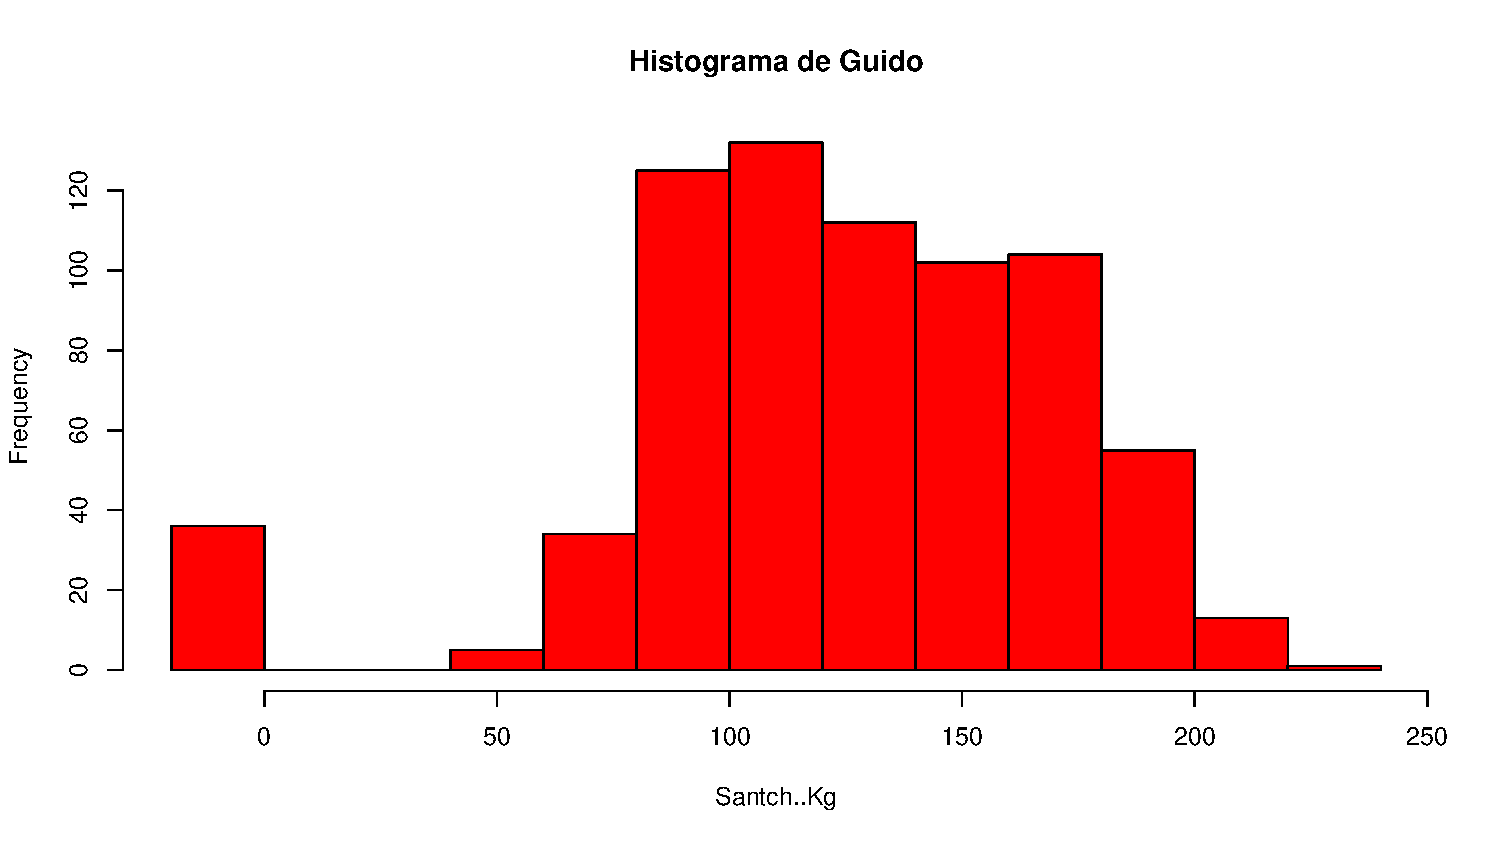
\includegraphics[width=\linewidth]{../Ejercicio-1/ImagenesEjercicio1/histSnatch.pdf}
	\caption{Histograma de la variable "Snatch..Kg".}	
	\label{fig:histSnatch}
\end{figure}
Es interesante observar el histograma, ya que revela dos aspectos distintos. Por un lado, se puede apreciar una distribución centrada alrededor de los 125 Kg, la cual muestra una forma de campana similar a una distribución normal. Por otro lado, se destacan una serie de valores en 0 Kg. Estos valores atípicos, conocidos como "outliers", no son representativos del rendimiento del atleta ni contribuyen a su predicción. Más bien, reflejan casos de atletas que no compitieron en esa categoría y se les asignó un valor de 0.
\subsection{Código utilizado}

\lstinputlisting[language=R]{../../../Code/Ej1a/Lambertucci_1.R}
%\end{document}
